\documentclass[pageno]{styles/jpaper}

\usepackage[normalem]{ulem}
\usepackage{listings}
\usepackage{color}
\usepackage{xspace}
\usepackage[title]{appendix}
\usepackage{tikz}
%\usepackage{pgf-pie}
\usepackage{tikz-qtree}
\usetikzlibrary{arrows,shapes,positioning,shadows,trees}
\usetikzlibrary{shadows,trees}
\usepackage{forest}



%replace XXX with the submission number you are given from the ASPLOS submission site.
\newcommand{\asplossubmissionnumber}{XXX}
\newcommand{\revisit}[1]{{\color{red} #1}}
\newcommand{\cmt}[1]{}

\newcommand{\uif}{uninterpreted functions}
\newcommand{\Strata}{{\tt Strata}\xspace}
\newcommand{\Stoke}{{\tt Stoke}\xspace}
\newcommand{\initS}{{\tt initial search}}
\newcommand{\secS}{{\tt secondary searches}}
\newcommand{\supp}{$2929$}
\newcommand{\total}{$3868$}
\newcommand{\unsupp}{$939$}
\newcommand{\K}{\ensuremath{\mathcal{{\tt K}}}\xspace}
\newcommand{\TS}[1]{{\tt #1}}
\newcommand{\instr}[1]{\texttt{#1}}
\newcommand{\opcode}[1]{\ensuremath{#1}}
\newcommand{\cond}[1]{\ensuremath{#1}}
\newcommand{\extract}{\emph{extract}\xspace}
\newcommand{\extractMInt}{\emph{extractMInt}\xspace}
\newcommand{\false}{\textbf{False}}
\newcommand{\true}{\textbf{True}}
\newcommand{\bool}{\texttt{Bool}\xspace}
\newcommand{\bv}{\texttt{Bitvector}\xspace}
\newcommand{\fig}[1]{\includegraphics[scale=.5]{#1}}
\newcommand{\reg}[1]{\emph{\%#1}}
\newcommand{\CF}[2]{$F_{#2}^{#1}$}
\newcommand{\GN}[2]{$G{[#2]}^{#1}$}

%%%%%% Immediates
\newcommand{\ImmUg}{$146$} % 118 + 28
\newcommand{\ImmTotal}{$308$}
\newcommand{\ImmG}{$190$}

%%%%%%% Registers
\newcommand{\RegTOTAL}{$1133$} % 1083 + 50
\newcommand{\RegSTRAT}{$742$} % 692 + 50
\newcommand{\RegSTOK}{$262$}
\newcommand{\RegMAN}{$129$}


\definecolor{codegreen}{rgb}{0,0.6,0}
\definecolor{codegray}{rgb}{0.5,0.5,0.5}
\definecolor{codepurple}{rgb}{0.58,0,0.82}
\definecolor{backcolour}{rgb}{0.95,0.95,0.92}
 
\lstdefinestyle{mystyle}{
    backgroundcolor=\color{backcolour},   
    commentstyle=\color{codegreen},
    keywordstyle=\color{magenta},
    numberstyle=\tiny\color{codegray},
    stringstyle=\color{codepurple},
    basicstyle=\footnotesize,
    breakatwhitespace=false,         
    breaklines=true,                 
    captionpos=b,                    
    keepspaces=true,                 
    numbers=left,                    
    numbersep=5pt,                  
    showspaces=false,                
    showstringspaces=false,
    showtabs=false,                  
    tabsize=2
}
\lstset{style=mystyle}

\begin{document}

\title{
A Complete Formal Semantics of User Level X86-64 Instruction Set}

\date{}
\maketitle

\thispagestyle{empty}

\begin{abstract}

\revisit{ToDo}

\end{abstract}

\section{Introduction}\label{sec:Intro}

\section{Preliminaries} \label{sec:Prilim}
In this section we will mention about two projects used extensively in our work. The first one is \K{}, , a semantics engineering tool in
which we chose to formalize our semantics. and the other is \Strata which we used to
obtain the semantics of individual X86-64 instructions.    

\subsection{Project Strata}

In order to get semantics of individual instructions, we build on top of project
\Strata~\cite{Heule2016a} which automatically synthesized formal semantics  of
the input/output behavior for $1796$ Haswell ISA X86-64 instructions. The key to
their results is stratified synthesis, where they use a set of instructions
whose semantics are known to synthesize the semantics of additional instructions
whose semantics are unknown. 
In a nutshell the approach is as follows. The approach needs as input  a small set of x86-64 instructions, the base set {\tt B}, whose semantics is already known. They execute
an instruction {\tt I} for which the formal semantics is not known yet on a set of test inputs {\tt TS} to obtain an initial description of its behavior. Then they search for a program {\tt p}, thats agrees with {\tt I} on T,  where {\tt p} only uses instructions drawn from the {\tt B}. This search will henceforth be referred as \initS{}. 



After that they perform multiple searches to get a set of programs {\tt P} all agreeing with {\tt I} on {\tt TS} and uses only the instructions from {\tt B}. These subseqent searches will henceforth be referred as \secS{}. Given two programs p, p$\prime$ $\in$ {\tt P}, they test whether $p\equiv_\text{Z3}p\prime$ using an SMT solver and the formulas from the base set. If the two programs are semantically distinct (meaning
the agreement on {\tt T} is coincidental), they know that one or both programs are not a correct description of {\tt I}. They use the model produced by the SMT solver to obtain an input {\tt t} that distinguishes $p$ and $p\prime$, add $t$ to the set of tests {\tt T}, and start over. This process is  repeated until they having enough programs according to a threshold. Once done, one {\tt p} $\in$ {\tt P} is chosen, according to some heuristics, and returned as the semantics of {\tt I}. Also {\tt p} is added to the base set {\tt B}.  This  enables stratified synthesis  as the vocabulary for expressing the semantics of more complex instructions expands.


Using this technique, they first came up with the semantics of $692$ register and
\revisit{$\sim120$} immediate instructions. The rest $\sim984$ are the immediate
and memory variants obtained by generalization of $692$ register instructions.     

\Strata uses \Stoke~\cite{Stoke2013} for the stochastic search step. \Stoke contains manually written formulas for a subset of the x86-64 instruction set, which \Strata uses to compare against the ones learned by stratification by asking an SMT solver if the formulas are equivalent.

\cmt{ 
    Using this combination of stochastic search + pruning
    using testing (we referred as {\tt initial search}) and subsequent refining of the
    search results using equivalence checking ({\tt henceforth referred as \secS{}
    }), }


\cmt{
    After having that {\tt initial search},
    they keep on searching  additional programs, called {\tt secondary
        searches}, each agreeing with {\tt I} on {\tt T} and using the instructions from {\tt B}, in a hope of
    getting  one which would prove non-equivalent to existing ones and
    thereby gaining more confidence on the searched programs. 
    
    In the process the initial set of test inputs got augmented by counter examples 
    
    and probably an
    augmented test-suite (as {\tt TS} might get augmented with a
    counter example from equivalence checker in the event of
    non-equivalence). 
}


\subsection{K Framework}


\section{X86-64 Instruction Semantics in \K} \label{sec:modelI}

\subsection{Modeling Instruction Semantics}
 
\begin{figure}[t]
    \centering
    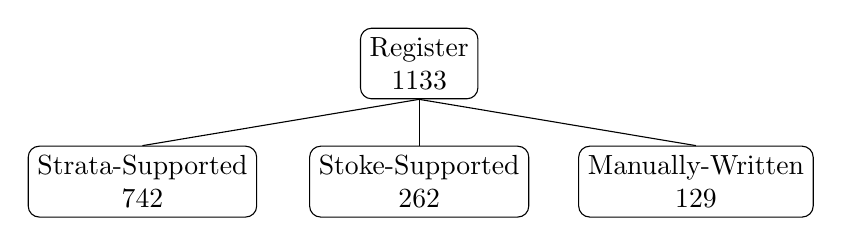
\begin{tikzpicture}
    [sibling distance=10em,
    every node/.style = {shape=rectangle, rounded corners,
        draw, align=center,
        top color=white\cmt{, bottom color=blue!20}}]]
    
    \node {Register\\ \RegTOTAL{}}
        child { node {Strata-Supported \\ \RegSTRAT{}} }
        child { node {Stoke-Supported \\ \RegSTOK{}} }
        child { node {Manually-Written \\ \RegMAN{}} };
    \end{tikzpicture}
    \caption{Distribution of register instructions}
    \label{fig-reg-dist}
\end{figure}


\tikzset{
    basic/.style  = {draw, text width=2cm, font=\sffamily, rectangle},
    root/.style   = {basic, rounded corners, thin, align=center\cmt{, fill=green!30}},
    level 2/.style = {basic, rounded corners, thin,align=center,  text width=8em},
    level 3/.style = {basic, thin, align=left, text width=6.5em}
}

\cmt{
\begin{figure*}[t]
    \centering
    \begin{tikzpicture}[
    level 1/.style={sibling distance=40mm},
    edge from parent/.style={->,draw},
    >=latex]
    
    % root of the the initial tree, level 1
    \node[root] {Immediates \\ \ImmTotal{}}
    % The first level, as children of the initial tree
    child {node[level 2] (c1) {Generalized}}
    child {node[level 2] (c1) {Generalized}}
    child {node[level 2] (c2) {Non-Generalized}};
    %child {node[level 2] (c3) {Drawing arrows between nodes}};
    
    
    \end{tikzpicture}
    \caption{Distribution of immediate instructions}
    \label{fig-imm-dist}
\end{figure*}
}

\begin{figure}[t]
\centering
\begin{tikzpicture}[
level 1/.style={sibling distance=40mm},
edge from parent/.style={->,draw},
>=latex]

% root of the the initial tree, level 1
\node[root] {Immediates \\ \ImmTotal{}}
% The first level, as children of the initial tree
child {node[level 2] (c1) {Generalized}}
child {node[level 2] (c2) {Non-Generalized}};
%child {node[level 2] (c3) {Drawing arrows between nodes}};

% The second level, relatively positioned nodes
\begin{scope}[every node/.style={level 3}]
\node [below of = c1, xshift=15pt] (c11) {Strata Supported};
\node [below of = c11] (c12) {Stoke Supported};
\node [below of = c12] (c13) {Manually Added};

\node [below of = c2, xshift=15pt] (c21) {Strata Supported};
\node [below of = c21] (c22) {Stoke Supported};
\node [below of = c22] (c23) {Manually Added};
\end{scope}

% lines from each level 1 node to every one of its "children"
\foreach \value in {1,2,3}
\draw[->] (c1.195) |- (c1\value.west);

\foreach \value in {1,2,3}
\draw[->] (c2.195) |- (c2\value.west);

\end{tikzpicture}
\caption{Distribution of immediate instructions}
\label{fig-imm-dist}
\end{figure}

In this work we supported formal semantics of the input/output behavior of
\supp{} out of \total{} x86-64 Haswell ISA instruction variants. Figure \ref{fig:IC} shows the classification of the instructions not supported using dotted ovals. The ones that are not supported can be categorized to System, Legacy mode, MMX, X87 and Cryptography instructions. Following are some of the immediate challenges that we needed to address.

\begin{enumerate}
    
    \item \textbf{CH.1: Supporting 
    \emph{un-stratified} Instructions} The paper ~\cite{Heule2016a} mentions that adding
    some primitive instructions (like saturated add) as the base instruction
    might help stratified more instructions. We would like to explore similar
    directions. Moreover, it would interesting if we can leverage the manually
    written instruction semantics from project \Stoke. \cmt{ and make sure to
        have the same correctness guarantee that \Strata provided in most of its
        cases.} 
           
    \item \textbf{CH.2: Getting Generic Formula for Immediates} The $\sim120$
    immediate instructions, mentioned above, do not have a corresponding
    register-only instruction to generalized from.  Therefore \Strata tries to
    learn a separate formula for every possible value of the 8 bit immediate
    operand.  We intend to have a more intuitive generic semantics (that works
        for all values of the immediate operand) for those instructions. 

 \item \textbf{CH.3: Modeling \emph{undef} flags} There are instructions which
 conditionally sets some cpu flags to \emph{undef}. For example, the shift left
 instruction \instr{salq \%cl, \%rbx} sets flag \reg{of} to \emph{undef} state
 if the count mask $>1$.  Also there are instructions like \instr{blsr \%eax,
   \%ebx} which un-conditionally puts flags like \reg{pf} \& \reg{af} into
   \emph{undef} state.
    
    \Strata while doing the {\tt initial search} does not test the flags which
    \emph{may} (for conditional \emph{undef}s)  or \emph{must} (for
        un-conditional \emph{undef}s) be taking undefined values. We intend to
    model the semantics of these flags with the same correctness guarantee as
    the other registers which do not result in \emph{undef} and hence modeled by
    \Strata.

    \item \textbf{CH.4: Modeling \reg{af} flag} \Strata chose not to model the
    \reg{af} flag as this is not commonly used. Supporting this flag fall within
    the scope of our work.
      
    \item \textbf{CH.5: Generalization to Immediate and Memory} How reliable is
    the generalization of register instructions to memory or immediate variants?
    \Strata states that the claim for the generalization is based on random
    testing.
    
    \item \textbf{CH.6: Formula simplification} In \Strata{}, formulas are added to the base set as soon as a specification has been learned (by learning multiple programs) and  the next target instruction, whose semantics is yet to be learned, uses the current base set to express its semantics. This implies that the target instructions  which comes later in the stratification process, might have complex formula (beyond the simplification rules that \Strata has). For example, the \Strata formula
    fir \instr{shrxl \%eax \%ebx \%ecx} contain around 2560 terms (excluding the operator symbols). 
    
    Moreover, for a non-floating point target instruction {\tt T}, \Strata might get a program containing floating point instructions (because the program agrees with T on a set of test inputs) which might result in a formula containing those floating point operations expressed in \uif{}.
    
    We intend to get a simpler and more intuitive formula in either cases. 
       
        

\end{enumerate} 

Following is a key observation concerning stratification which help us handle
the most of the above mentioned challenges.

\paragraph{Observation} In order to get the semantics of a target instruction
{\tt I}, \Strata uses \Stoke along with a set {\tt TS} of $6580$ test cases to
synthesize an instruction sequence which agrees with {\tt I} on {\tt TS} (which
    means the output behavior of the instruction sequence matches with that on
    real hardware for input {\tt TS}). After having that {\tt initial search},
           they keep on searching  additional sequences, called {\tt secondary
             searches}, each agreeing with {\tt I} on {\tt TS}, in a hope of
             getting  one which would prove non-equivalent to existing ones and
             thereby gaining more confidence on the search and probably an
             augmented test-suite (as {\tt TS} might get augmented with a
                 counter example from equivalence checker in the event of
                 non-equivalence). 
      
      One unfavorable possibility for \Strata is when all subsequent secondary
      search results proves  equivalent to the one obtained from initial search
      and hence there are no conflicts among searches, in which case it  means
      that  secondary searches fail to add any ``confidence'' to the initial
      search result and end up giving the same correctness guarantee as provided
      by the initial search result. Even though in such unfavorable case, the
      secondary searches might have provided ``better'' choices to pick the
      final formula from. A better choice of formula do not contain
      uninterpreted functions or  non-linear arithmetics and are simple.  
    
   In the paper\cite{Heule2016a}, it is mentioned that there are only $50$
   cases, where they found a (valid) counterexample. That means, there are $762
   = (692 + 120 - 50)$ instructions, for which  the initial stoke search using
   augmented test-suite, containing $6630\ (= 6580 + 50$) tests,  is sufficient
   enough to provide a semantics with the same correctness guarantee which
   \Strata provides.   In other words, in  most of the cases, the correctness
   guarantee of secondary searches is same as that of the initial stoke search
   using the augmented test-suite (henceforth referred as {\tt ATS})  which
   \Strata ends up with. \revisit{Had \Strata supported rest of the instructions 
       it could have performed better by providing more counter examples. 
       In that sense can we generalize the the observation to unsupported ones?}
      
      
    \paragraph{Handling CH.1} For an unsupported instruction {\tt I}, we either
    model its semantics  manually or borrowed it from project \Stoke.   Once we
    have this candidate, we test it against hardware using {\tt ATS}.  Once the
    test passes we claim (from the above observation) the semantics to have the
    same correctness guarantee which \Strata provided for most of its cases.
    
    This helped us finding instruction semantics bugs in Intel
    Manual~\cite{BugIntel} and \Stoke~\cite{BugStoke983}.
    
    We understand that this is not as efficient as \Stoke, which is fully
    automatic in getting these formulas, and we do not intend to make any
    contribution towards efficient generation of instruction semantics. The
    purpose of above mentioned effort is to deliver in cases where \Stoke cannot
    without loosing much on the correctness guarantee. 
   
   Moreover, writing the semantics manually might alleviate the need of
   secondary search as a means to provide ``better'' formula as we can control
   the complexity and choice of operations to include in the formula. Also
   carefully written manual formula tend to need less number of conflicting
   searches than the onces generated by random search engines like Stoke.
   
   We also tried the following other options, which we do not pursue further:
   \begin{itemize}
       \item \textbf{Augmenting the Base Set: }
       Coming up with a suitable set of base instructions, which help 
       synthesizing the semantics most of the user level instruction, could be framed 
       as an optimization problem, which we do not explore in this work. \revisit{Why?} 
       
       \item \textbf{Reducing \Stoke Search Space: }This option is based
       on the observation that {\tt initial search} for some instructions (like
       \instr{vfmaddsub132pd \%ymm1 \%ymm2 \%ymm3}) times-out because of the
       huge search space to be explored by \Stoke. We tried to limit the search
       space using manually learned heuristics. An example of one such heuristic is
       \emph{ If we know the semantics of an instruction with ymm operands and the
           target instruction, which we want to learn, is a variant of that
           instruction and uses xmm operand, then the search pool should contain
           some specific instructions}. This particular heuristic  work well for few
       instructions. In the general case, getting the search pool for every
       target instruction, need an approximate insight about the semantics of
       the target instructions itself. Even though such information is available
       in manuals but we find it difficult to extract it in a way to create the
       search pool, which is the main reason we drop this venture.
   \end{itemize} 
    
   
   
   
   
   \paragraph{Handling CH.2} The instructions in this category either  have a
   separate formula for all or some of 256 possible values. We refer each of the
   separate formulas for instruction {\tt I} as a concrete formula \CF{I}{c} for
   a particular constant value {\tt c} of immediate operand.  In either case, we
   get a generic formula, $G^I$ either by writing it manually or borrowing it
   from  \Stoke project.
   
   In the case where we have a separate \CF{I}{c} $\forall c \in \{0...255\}$,
   we do a Z3 equivalence check as follows: $\forall c \in \{0..255\}:$
   \CF{I}{c} $\equiv_\text{Z3}$ \GN{I}{c}, where \GN{I}{c} is obtained by
   replacing the symbolic inputs of $G^I$ with constant value {\tt c}. A
   successful equivalence check suggest $G^I$ to be a generic formula with the
   same correctness guarantee that \Strata has for any of the individual
   concrete formulas. For the case where we have a separate formula for a subset
   of constant values, we do the same equivalence check as before for that
   subset. The constants for which we do not have a separate formula we test
   \GN{I}{c} using {\tt ATS}, the final augmented test-suite of \Strata. 
    
    \paragraph{Handling CH.3} There are $474\ (= 141(\text{Reg}) +
        109(\text{Imm}) + 224(\text{Mem}))$ instructions that results in
    conditional  (or \emph{may}) \emph{undef} ($162\ (= 40 + 46 + 76)$) or
    un-conditional (or \emph{must}) \emph{undef} ($312\ (= 101 + 63 + 148)$)  in
    one or more cpu flag.  The semantics of most of the cpu flags (which
        \emph{may} or \emph{must} take \emph{undef} values) are already modeled
    in \Stoke. We needed to model the semantics of flag registers for $40$
    instructions involving {\tt shifts, rotates}~\cite{BugStoke986}. 
    
    For \emph{may undef} cases, we tested against hardware, using {\tt ATS}, for
    the scenarios when the condition for undefinedness is not triggered.  For
    the remaining cases, (1) \emph{may undef}s where the condition for
    triggering \emph{undef} is true and (2) \emph{must undef}, we make sure that
    \K execution halts when the undefinedness condition is triggered. This help
    is find bugs in the \Stoke implementation of $8$
    instructions~\cite{BugStoke986} ( Note that these $8$ instructions are not
        stratified and hence we borrowed it from \Stoke).   
    
    
   \paragraph{Handling CH.4}
   \begin{figure}[t]
       \centering
       \fig{figures/af_distribution.eps}
       \caption{Instructions affecting \reg{af} flag.} The numbers represent count of (Register/Immediate/Memory) Instructions. 
       \label{fig:AD}
   \end{figure}

   Figure \ref{fig:AD} represents the distribution of instructions affecting the
   \reg{af} flag in a defined or un-defined way (which could be conditional or
       un-conditional).  We tested all the instructions for the defined cases
   using {\tt ATS}. For conditionally undefined cases, we tested for the
   scenarios when the condition for undefinedness is not triggered.  For all
   remaining cases,  we make sure that the \K execution halts when the
   undefinedness condition is triggered.        
   
   \paragraph{Handling CH.5}
   
   While testing we found instructions like \instr{movss xmm m64, movsd xmm 64}
   where the generalization from the corresponding register variant is not
   faithful. Followings are the semantics of \instr{movsd xmm1, xmm2} and its
   memory variant  \instr{movsd xmm1, m64}. Clearly, the memory variant cannot
   be obtained using generalization of the  corresponding register instruction.   
   
   {\small \tt 
       \centering
       \begin{tabular}[b]{l}
           // movsd xmm1, xmm2 \\
           S1. DEST[63:0] $\leftarrow$ SRC[63:0] \\ 
           S2. DEST[MAXVL-1:64] (Unmodified) \\
           \\
           // movsd xmm1, m64 \\
           S1. DEST[63:0] $\leftarrow$ SRC[63:0] \\
           S2. DEST[MAXVL-1:64] $\leftarrow$ 0 \\
       \end{tabular}
   }





\cmt{
   
\subsection{Porting to \K Rules}

For the purpose of getting  \K rules, we could have directly converted the
\Strata formulas for an instruction to \K rule assuming that the \Strata's
symbolic execution over the stratified instruction sequence is correct.

Given that fact the \K's symbolic execution engine is more trusted as that has
been used extensively in language-agnostic manner to perform symbolic execution,
     we decided to use \K's symbolic executor. Also in order to check if
     \Strata's symbolic execution engine is correct, we did an equivalence check
     on the outputs of both the symbolic executions.   
 

\begin{enumerate}
\item Implementing the base instructions semantics in \K and testing them.
\item Symbolic execution of the stratified instruction sequences.
\item Dealing with scratch pad registers.
\item Equivalence check between \Strata formula ad the output of 2.
   
   All the checks are \emph{unsat}, expect one where the check fail to due a bug
   in the simplification rules in \Strata, which states the following lemma
   related to two single precision floating point numbers  {\tt A}  and {\tt B},
   which is not correct for {\tt NaNs}. However this bug is fixed in the latest
   version of \Stoke. 
   
   
   { \tt  
        \begin{tabular}[b]{l}
   \qquad sub\_single(A, B) $\equiv$ 0 if A == B     
      \end{tabular}
  }
   
\item {Simplification of formulas:} Simplification generates simple \K rule
(sometimes simpler than the corresponding \Strata formula).  Also it is much
easier to write the simplification rules in \K.\revisit{show the example for
  concat(A[1:2], concate(B[2:3], X)) $\equiv$ concate(A[1:3], X)}


\item One drawback of the \Strata formulas is they could be non-intuitive and
complex at times when the simplification rules are not adequate enough to
simplify their complexity to more intuitive formulas. Appendix \ref{sec:AP:A}
provides such an example.  Towards the goal of having intuitive formulas, we
borrowed the hand written formula (provided they are simpler) from \Stoke or
manually write those  and check equivalence with the stratified formula. If they
match on all register state and/or memory, we employ that in our \K semantics.

\cmt{
An example of one such simplification opportunity is: 
     { \tt  
      \begin{tabular}[b]{l}
          ($0_{32}$ $\cdot$ \%rax[32:0]) $\oplus$ \%rax $\equiv$ \%rax[63:32] $\cdot$  $0_{32}$ 
      \end{tabular}
    }
}

       


\end{enumerate}

\subsection{Supporting un-stratified instructions \& Porting their formulas to \K Rules}

\subsubsection{Supporting un-stratified instructions}
\paragraph{Instruction support status}



\subsection{Porting to \K Rules}

\Strata could output the internal AST, used to model a register state formula, in different
formats. Supported backend are SmtLib and Prefix notation. We have added another backend 
to generate \K rule. We need some way to validate the backend. 

\paragraph{Validate the Backend}

The \K rules generated using the backend are matched (syntactically)  against
the ones we already obtained via symbolic execution on stratified instructions.
Other than validaing the backend, this has an added benefit that in order to get
the exact match, we need to port all the simplification rules from \K to strata
code, which in turn will later help in generating simplified \K rules for
non-stratified instructions. 

Main challenges in getting an exact match are:
\begin{itemize}

\item  \Strata rules uses \extract to extract portion of a bit-vector. The high
and low indices of \extract are obtained considering LSB at index 0, whereas \K
uses \extractMInt for the same purpose, but uses MSB at index zero.

\item  \Strata uses flags as \bool, whereas they are treated as \bv in our
semantics. We modifed strata so as to treat flag registers as 1 bit bitvectors.

\end{itemize}

}

\section{Evaluation} \label{sec:Eval}

\section{Application} \label{sec:Appl}

\section{Related Work}\label{sec:RW}




\begin{appendices}
\section{An Example of \Strata Formula}\label{sec:AP:A}

Following is the \Strata formula for an instruction \instr{vpxor \%ymm3, \%ymm2, \%ymm1},


\begin{lstlisting}[language=Java]

(let ((a!1 (bvxor ((_ extract 255 192) ymm3)
                  ((_ extract 255 192) ymm2)
                  (bvor ((_ extract 255 192) ymm3)
                        (bvxor ((_ extract 255 192) ymm3)
                               ((_ extract 255 192) ymm2)))))
      (a!3 (bvxor ((_ extract 191 128) ymm3)
                  ((_ extract 191 128) ymm2)
                  (bvor ((_ extract 191 128) ymm3)
                        (bvxor ((_ extract 191 128) ymm3)
                               ((_ extract 191 128) ymm2)))))
      (a!5 (bvxor ((_ extract 127 64) ymm3)
                  ((_ extract 127 64) ymm2)
                  (bvor ((_ extract 127 64) ymm3)
                        (bvxor ((_ extract 127 64) ymm3)
                               ((_ extract 127 64) ymm2)))))
      (a!7 (bvxor ((_ extract 63 0) ymm3)
                  ((_ extract 63 0) ymm2)
                  (bvor ((_ extract 63 0) ymm3)
                        (bvxor ((_ extract 63 0) ymm3) ((_ extract 63 0) ymm2))))))
(let ((a!2 (bvxor ((_ extract 255 192) ymm3)
                  ((_ extract 255 192) ymm2)
                  (bvor ((_ extract 255 192) ymm3)
                        (bvxor ((_ extract 255 192) ymm3)
                               ((_ extract 255 192) ymm2)))
                  (bvor a!1
                        ((_ extract 255 192) ymm2)
                        ((_ extract 255 192) ymm3))))
      (a!4 (bvxor ((_ extract 191 128) ymm3)
                  ((_ extract 191 128) ymm2)
                  (bvor ((_ extract 191 128) ymm3)
                        (bvxor ((_ extract 191 128) ymm3)
                               ((_ extract 191 128) ymm2)))
                  (bvor a!3
                        ((_ extract 191 128) ymm2)
                        ((_ extract 191 128) ymm3))))
      (a!6 (bvxor ((_ extract 127 64) ymm3)
                  ((_ extract 127 64) ymm2)
                  (bvor ((_ extract 127 64) ymm3)
                        (bvxor ((_ extract 127 64) ymm3)
                               ((_ extract 127 64) ymm2)))
                  (bvor ((_ extract 127 64) ymm2) ((_ extract 127 64) ymm3) a!5)))
      (a!8 (bvxor ((_ extract 63 0) ymm3)
                  ((_ extract 63 0) ymm2)
                  (bvor ((_ extract 63 0) ymm3)
                        (bvxor ((_ extract 63 0) ymm3) ((_ extract 63 0) ymm2)))
                  (bvor ((_ extract 63 0) ymm2) ((_ extract 63 0) ymm3) a!7))))
  (concat a!2 a!4 a!6 a!8)))
\end{lstlisting}

where as following is the formula obtained from \Stoke (hand-written) and 
 Z3 took $88.70$ secs to prove that they are equivalent.

\begin{lstlisting}[language=Java]
%ymm1  : (bvxor %ymm2 %ymm3)
\end{lstlisting}
\end{appendices}


\bibliographystyle{plain}
\bibliography{bibs/references,bibs/modeling-X86-semantics,bibs/bugs}


\end{document}

\grid
\grid
